\begin{exercise}
      {ID-11355ef27a46bdeef9e283bbbd480a94e14eb326}
      {Parallelogramm}
  \ifproblem\problem
    Gegeben sei ein beliebiges (konvexes) Viereck. Zerschneide es so in vier
    kleinere Vierecke, dass man daraus ein (gleich großes) Parallelogramm legen
    kann.
  \fi
  %\ifoutline\outline
  %\fi
  \ifoutcome\outcome
    Man muss das Viereck von der Mitte einer Seite zur Mitte der
    gegenüberliegenden Seite zerschneiden:
    \begin{center}
      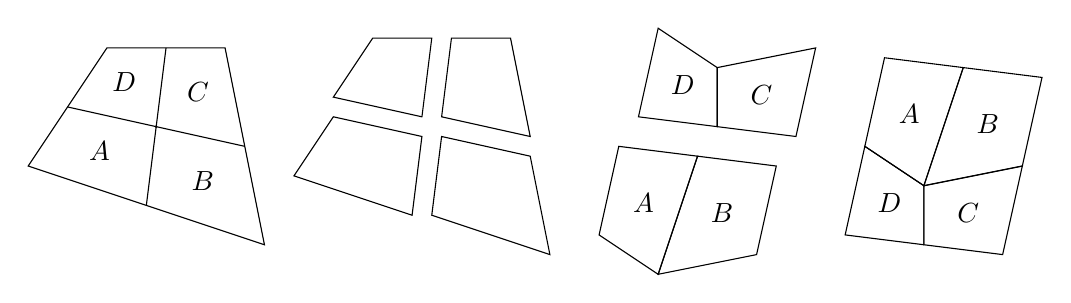
\begin{tikzpicture}[scale=0.5]
        \begin{scope}
          \coordinate (A)   at (-3.0000, -1.0000);
          \coordinate (B)   at ( 3.0000, -3.0000);
          \coordinate (C)   at ( 2.0000,  2.0000);
          \coordinate (D)   at (-1.0000,  2.0000);
          \coordinate (M1)  at ( 0.0000, -2.0000);
          \coordinate (M2)  at ( 2.5000, -0.5000);
          \coordinate (M3)  at ( 0.5000,  2.0000);
          \coordinate (M4)  at (-2.0000,  0.5000);
          \coordinate (M)   at ( 0.2500,  0.0000);
          \coordinate (MA)  at (-1.1875, -0.6250);
          \coordinate (MB)  at ( 1.4375, -1.3750);
          \coordinate (MC)  at ( 1.3125,  0.8750);
          \coordinate (MD)  at (-0.5625,  1.1250);
          \coordinate (MMA) at ( 0.2500,  0.0000);
          \coordinate (MMB) at ( 0.2500,  0.0000);
          \coordinate (MMC) at ( 0.2500,  0.0000);
          \coordinate (MMD) at ( 0.2500,  0.0000);
          \coordinate (M1A) at ( 0.0000, -2.0000);
          \coordinate (M1B) at ( 0.0000, -2.0000);
          \coordinate (M2B) at ( 2.5000, -0.5000);
          \coordinate (M2C) at ( 2.5000, -0.5000);
          \coordinate (M3C) at ( 0.5000,  2.0000);
          \coordinate (M3D) at ( 0.5000,  2.0000);
          \coordinate (M4D) at (-2.0000,  0.5000);
          \coordinate (M4A) at (-2.0000,  0.5000);
          \draw (A) -- (B) -- (C) -- (D) -- cycle;
          \draw (M1) -- (M3) (M2) -- (M4);
          \fill (M)  circle[radius=1pt];
          \node at (MA) {$A$};
          \node at (MB) {$B$};
          \node at (MC) {$C$};
          \node at (MD) {$D$};
        \end{scope}
        \begin{scope}[xshift=7cm]
          \coordinate (A)   at (-3.2500, -1.2500);
          \coordinate (B)   at ( 3.2500, -3.2500);
          \coordinate (C)   at ( 2.2500,  2.2500);
          \coordinate (D)   at (-1.2500,  2.2500);
          \coordinate (M1)  at ( 0.0000, -2.0000);
          \coordinate (M2)  at ( 2.5000, -0.5000);
          \coordinate (M3)  at ( 0.5000,  2.0000);
          \coordinate (M4)  at (-2.0000,  0.5000);
          \coordinate (M)   at ( 0.2500,  0.0000);
          \coordinate (MA)  at (-1.4375, -0.8750);
          \coordinate (MB)  at ( 1.6875, -1.6250);
          \coordinate (MC)  at ( 1.5625,  1.1250);
          \coordinate (MD)  at (-0.8125,  1.3750);
          \coordinate (MMA) at ( 0.0000, -0.2500);
          \coordinate (MMB) at ( 0.5000, -0.2500);
          \coordinate (MMC) at ( 0.5000,  0.2500);
          \coordinate (MMD) at ( 0.0000,  0.2500);
          \coordinate (M1A) at (-0.2500, -2.2500);
          \coordinate (M1B) at ( 0.2500, -2.2500);
          \coordinate (M2B) at ( 2.7500, -0.7500);
          \coordinate (M2C) at ( 2.7500, -0.2500);
          \coordinate (M3C) at ( 0.7500,  2.2500);
          \coordinate (M3D) at ( 0.2500,  2.2500);
          \coordinate (M4D) at (-2.2500,  0.7500);
          \coordinate (M4A) at (-2.2500,  0.2500);
          \draw (A) -- (M1A) -- (MMA) -- (M4A) -- cycle;
          \draw (B) -- (M2B) -- (MMB) -- (M1B) -- cycle;
          \draw (C) -- (M3C) -- (MMC) -- (M2C) -- cycle;
          \draw (D) -- (M4D) -- (MMD) -- (M3D) -- cycle;
          \node at (MA) {$\curvearrowleft$};
          \node at (MB) {$\curvearrowright$};
          \node[rotate=180] at (MC) {$\curvearrowleft$};
          \node[rotate=180] at (MD) {$\curvearrowright$};
        \end{scope}
        \begin{scope}[xshift=14cm]
          \coordinate (A)   at (-1.0000, -3.7500);
          \coordinate (B)   at (-1.0000, -3.7500);
          \coordinate (C)   at ( 0.5000,  1.5000);
          \coordinate (D)   at ( 0.5000,  1.5000);
          \coordinate (M1)  at ( 0.0000, -2.0000);
          \coordinate (M2)  at ( 2.5000, -0.5000);
          \coordinate (M3)  at ( 0.5000,  2.0000);
          \coordinate (M4)  at (-2.0000,  0.5000);
          \coordinate (M)   at ( 0.2500,  0.0000);
          \coordinate (MA)  at (-1.3750, -1.9375);
          \coordinate (MB)  at ( 0.6250, -2.1875);
          \coordinate (MC)  at ( 1.6250,  0.8125);
          \coordinate (MD)  at (-0.3750,  1.0625);
          \coordinate (MMA) at (-2.0000, -0.5000);
          \coordinate (MMB) at ( 2.0000, -1.0000);
          \coordinate (MMC) at ( 2.5000, -0.2500);
          \coordinate (MMD) at (-1.5000,  0.2500);
          \coordinate (M1A) at ( 0.0000, -0.7500);
          \coordinate (M1B) at ( 0.0000, -0.7500);
          \coordinate (M2B) at ( 1.5000, -3.2500);
          \coordinate (M2C) at ( 3.0000,  2.0000);
          \coordinate (M3C) at ( 0.5000,  0.0000);
          \coordinate (M3D) at ( 0.5000,  0.0000);
          \coordinate (M4D) at (-1.0000,  2.5000);
          \coordinate (M4A) at (-2.5000, -2.7500);
          \draw (A) -- (M1A) -- (MMA) -- (M4A) -- cycle;
          \draw (B) -- (M2B) -- (MMB) -- (M1B) -- cycle;
          \draw (C) -- (M3C) -- (MMC) -- (M2C) -- cycle;
          \draw (D) -- (M4D) -- (MMD) -- (M3D) -- cycle;
          \node at (MA) {$A$};
          \node at (MB) {$B$};
          \node at (MC) {$C$};
          \node at (MD) {$D$};
        \end{scope}
        \begin{scope}[xshift=21cm]
          \coordinate (A)   at (-1.2500, -1.5000);
          \coordinate (B)   at (-1.2500, -1.5000);
          \coordinate (C)   at (-1.2500, -1.5000);
          \coordinate (D)   at (-1.2500, -1.5000);
          \coordinate (M1)  at ( 0.0000, -2.0000);
          \coordinate (M2)  at ( 2.5000, -0.5000);
          \coordinate (M3)  at ( 0.5000,  2.0000);
          \coordinate (M4)  at (-2.0000,  0.5000);
          \coordinate (M)   at ( 0.2500,  0.0000);
          \coordinate (MA)  at (-1.6250,  0.3125);
          \coordinate (MB)  at ( 0.3750,  0.0625);
          \coordinate (MC)  at (-0.1250, -2.1875);
          \coordinate (MD)  at (-2.1250, -1.9375);
          \coordinate (MMA) at (-2.2500,  1.7500);
          \coordinate (MMB) at ( 1.7500,  1.2500);
          \coordinate (MMC) at ( 0.7500, -3.2500);
          \coordinate (MMD) at (-3.2500, -2.7500);
          \coordinate (M1A) at (-0.2500,  1.5000);
          \coordinate (M1B) at (-0.2500,  1.5000);
          \coordinate (M2B) at ( 1.2500, -1.0000);
          \coordinate (M2C) at ( 1.2500, -1.0000);
          \coordinate (M3C) at (-1.2500, -3.0000);
          \coordinate (M3D) at (-1.2500, -3.0000);
          \coordinate (M4D) at (-2.7500, -0.5000);
          \coordinate (M4A) at (-2.7500, -0.5000);
          \draw (A) -- (M1A) -- (MMA) -- (M4A) -- cycle;
          \draw (B) -- (M2B) -- (MMB) -- (M1B) -- cycle;
          \draw (C) -- (M3C) -- (MMC) -- (M2C) -- cycle;
          \draw (D) -- (M4D) -- (MMD) -- (M3D) -- cycle;
          \node at (MA) {$A$};
          \node at (MB) {$B$};
          \node at (MC) {$C$};
          \node at (MD) {$D$};
        \end{scope}
      \end{tikzpicture}
    \end{center}
  \fi
\end{exercise}
